\documentclass{standalone}
\usepackage{graphicx}	
\usepackage{amssymb, amsmath}
\usepackage{color}

\usepackage{tikz}
\usetikzlibrary{intersections, backgrounds}

\definecolor{light}{RGB}{220, 188, 188}
\definecolor{mid}{RGB}{185, 124, 124}
\definecolor{dark}{RGB}{143, 39, 39}
\definecolor{highlight}{RGB}{180, 31, 180}
\definecolor{gray10}{gray}{0.1}
\definecolor{gray20}{gray}{0.2}
\definecolor{gray30}{gray}{0.3}
\definecolor{gray40}{gray}{0.4}
\definecolor{gray60}{gray}{0.6}
\definecolor{gray70}{gray}{0.7}
\definecolor{gray80}{gray}{0.8}
\definecolor{gray90}{gray}{0.9}
\definecolor{gray95}{gray}{0.95}

\newcommand*{\offset}{0.025}

\begin{document}

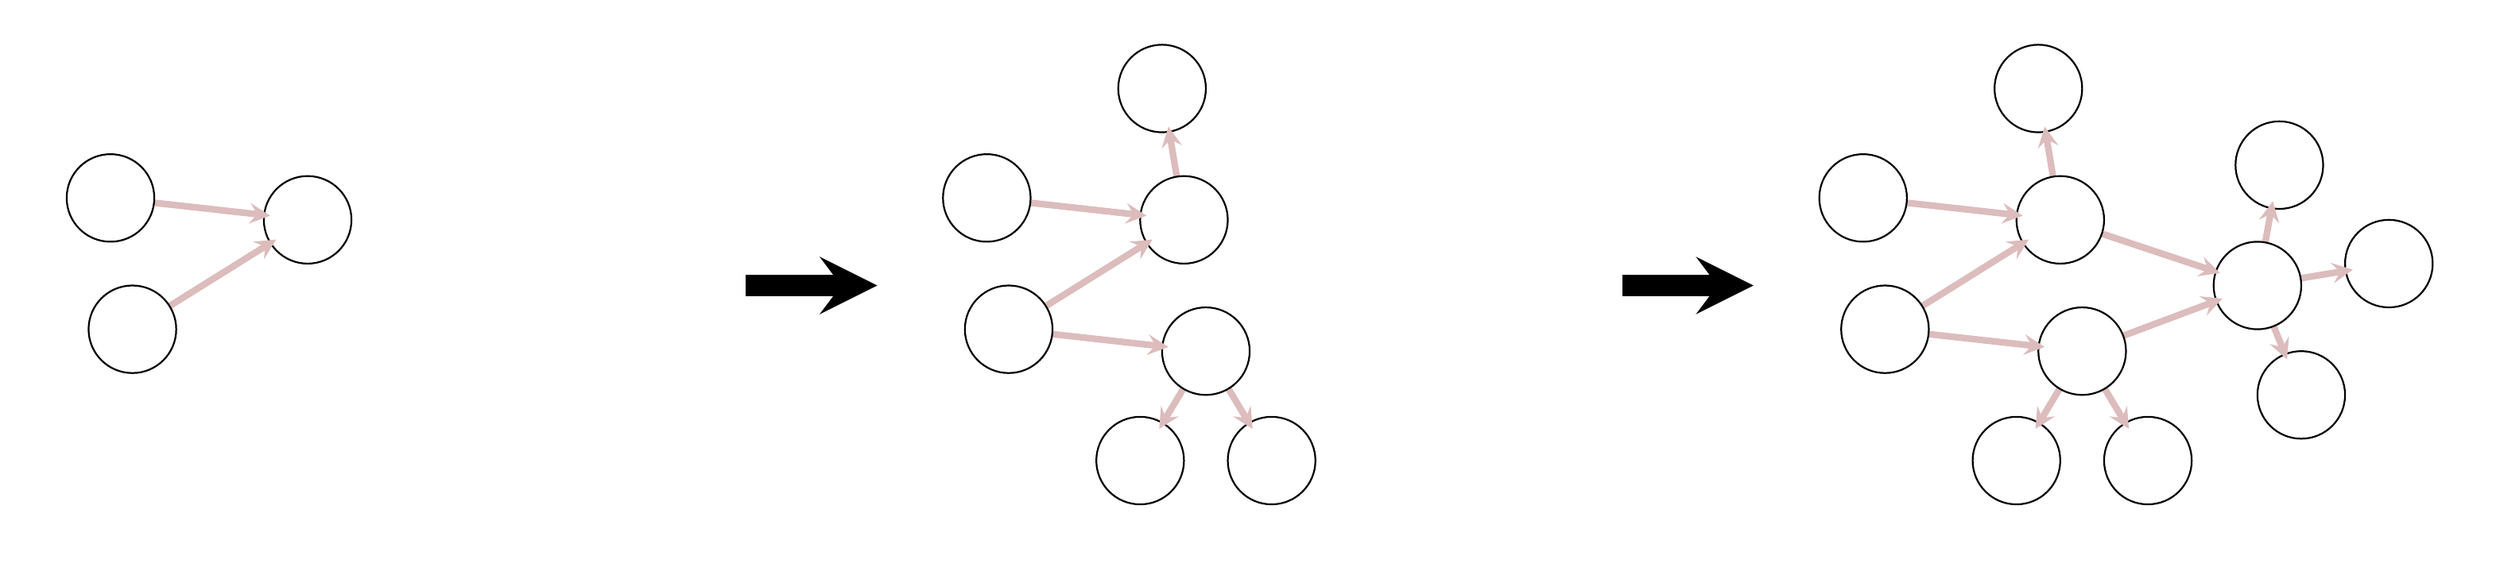
\begin{tikzpicture}[scale=0.35, thick]
  % One
  \draw [color=white] (-56, -12) rectangle +(32, 24);
  
  %\filldraw [fill=white] (7 - 40, 5.5) circle (2);
  
  %\filldraw [fill=white] (8 - 40, -5) circle (2);
  
  %\filldraw [fill=white] (12 - 40, 1) circle (2);
  
  %\draw [->, >=stealth, line width=3, color=light] (6 - 40, 0) -- +(1 * 0.7, 5.5 * 0.7);
  %\draw [->, >=stealth, line width=3, color=light] (6 - 40, 0) -- +(2 * 0.675, -5 * 0.675);
  %\draw [->, >=stealth, line width=3, color=light] (6 - 40, 0) -- +(6 * 0.725, 1 * 0.725);
  %\filldraw [fill=white] (6 - 40, 0) circle (2);
  
  %\filldraw [fill=white] (1 - 40, -8) circle (2);
  
  %\filldraw [fill=white] (-5 - 40, -8) circle (2);

  %\draw [->, >=stealth, line width=3, color=light] (-2 - 40, -3) -- +(3 * 0.71, -5 * 0.71);
  %\draw [->, >=stealth, line width=3, color=light] (-2 - 40, -3) -- +(-3 * 0.71, -5 * 0.71);
  %\draw [->, >=stealth, line width=3, color=light] (-2 - 40, -3) -- +(8 * 0.8, 3 * 0.8);
  %\filldraw [fill=white] (-2 - 40, -3) circle (2);
  
  %\filldraw [fill=white] (-4 - 40, 9) circle (2);
  
  %\draw [->, >=stealth, line width=3, color=light] (-3 - 40, 3) -- +(-1 * 0.71, 6 * 0.71);
  %\draw [->, >=stealth, line width=3, color=light] (-3 - 40, 3) -- +(9 * 0.81, -3 * 0.81);
  \filldraw [fill=white] (-3 - 40, 3) circle (2);
  
  \draw [->, >=stealth, line width=3, color=light] (-11 - 40, -2) -- +(8 * 0.82, 5 * 0.82);
  %\draw [->, >=stealth, line width=3, color=light] (-11 - 40, -2) -- +(9 * 0.81, -1 * 0.81);
  \filldraw [fill=white] (-11 - 40, -2) circle (2);
  
  \draw [->, >=stealth, line width=3, color=light] (-12 - 40, 4) -- +(9 * 0.81, -1 * 0.81);
  \filldraw [fill=white] (-12 - 40, 4) circle (2);
  
  \draw [->, >=stealth, line width=10, color=black] (-23, 0) -- +(6, 0);
  
  % Two
  \draw [color=white] (-16, -12) rectangle +(32, 24);
  
  %\filldraw [fill=white] (7, 5.5) circle (2);
  
  %\filldraw [fill=white] (8, -5) circle (2);
  
  %\filldraw [fill=white] (12, 1) circle (2);
  
  %\draw [->, >=stealth, line width=3, color=light] (6, 0) -- +(1 * 0.7, 5.5 * 0.7);
  %\draw [->, >=stealth, line width=3, color=light] (6, 0) -- +(2 * 0.675, -5 * 0.675);
  %\draw [->, >=stealth, line width=3, color=light] (6, 0) -- +(6 * 0.725, 1 * 0.725);
  %\filldraw [fill=white] (6, 0) circle (2);
  
  \filldraw [fill=white] (1, -8) circle (2);
  
  \filldraw [fill=white] (-5, -8) circle (2);

  \draw [->, >=stealth, line width=3, color=light] (-2, -3) -- +(3 * 0.71, -5 * 0.71);
  \draw [->, >=stealth, line width=3, color=light] (-2, -3) -- +(-3 * 0.71, -5 * 0.71);
  %\draw [->, >=stealth, line width=3, color=light] (-2, -3) -- +(8 * 0.8, 3 * 0.8);
  \filldraw [fill=white] (-2, -3) circle (2);
  
  \filldraw [fill=white] (-4, 9) circle (2);
  
  \draw [->, >=stealth, line width=3, color=light] (-3, 3) -- +(-1 * 0.71, 6 * 0.71);
  %\draw [->, >=stealth, line width=3, color=light] (-3, 3) -- +(9 * 0.81, -3 * 0.81);
  \filldraw [fill=white] (-3, 3) circle (2);
  
  \draw [->, >=stealth, line width=3, color=light] (-11, -2) -- +(8 * 0.82, 5 * 0.82);
  \draw [->, >=stealth, line width=3, color=light] (-11, -2) -- +(9 * 0.81, -1 * 0.81);
  \filldraw [fill=white] (-11, -2) circle (2);
  
  \draw [->, >=stealth, line width=3, color=light] (-12, 4) -- +(9 * 0.81, -1 * 0.81);
  \filldraw [fill=white] (-12, 4) circle (2);
  
  \draw [->, >=stealth, line width=10, color=black] (17, 0) -- +(6, 0);
  
  % Three
  \draw [color=white] (-16 + 40, -12) rectangle +(32, 24);
  
  \filldraw [fill=white] (7 + 40, 5.5) circle (2);
  
  \filldraw [fill=white] (8 + 40, -5) circle (2);
  
  \filldraw [fill=white] (12 + 40, 1) circle (2);
  
  \draw [->, >=stealth, line width=3, color=light] (6 + 40, 0) -- +(1 * 0.7, 5.5 * 0.7);
  \draw [->, >=stealth, line width=3, color=light] (6 + 40, 0) -- +(2 * 0.675, -5 * 0.675);
  \draw [->, >=stealth, line width=3, color=light] (6 + 40, 0) -- +(6 * 0.725, 1 * 0.725);
  \filldraw [fill=white] (6 + 40, 0) circle (2);
  
  \filldraw [fill=white] (1 + 40, -8) circle (2);
  
  \filldraw [fill=white] (-5 + 40, -8) circle (2);

  \draw [->, >=stealth, line width=3, color=light] (-2 + 40, -3) -- +(3 * 0.71, -5 * 0.71);
  \draw [->, >=stealth, line width=3, color=light] (-2 + 40, -3) -- +(-3 * 0.71, -5 * 0.71);
  \draw [->, >=stealth, line width=3, color=light] (-2 + 40, -3) -- +(8 * 0.8, 3 * 0.8);
  \filldraw [fill=white] (-2 + 40, -3) circle (2);
  
  \filldraw [fill=white] (-4 + 40, 9) circle (2);
  
  \draw [->, >=stealth, line width=3, color=light] (-3 + 40, 3) -- +(-1 * 0.71, 6 * 0.71);
  \draw [->, >=stealth, line width=3, color=light] (-3 + 40, 3) -- +(9 * 0.81, -3 * 0.81);
  \filldraw [fill=white] (-3 + 40, 3) circle (2);
  
  \draw [->, >=stealth, line width=3, color=light] (-11 + 40, -2) -- +(8 * 0.82, 5 * 0.82);
  \draw [->, >=stealth, line width=3, color=light] (-11 + 40, -2) -- +(9 * 0.81, -1 * 0.81);
  \filldraw [fill=white] (-11 + 40, -2) circle (2);
  
  \draw [->, >=stealth, line width=3, color=light] (-12 + 40, 4) -- +(9 * 0.81, -1 * 0.81);
  \filldraw [fill=white] (-12 + 40, 4) circle (2);
\end{tikzpicture}

\end{document}  